%. Introduction
%  Adsorbate-Metal systems 
%      catalysts
%      devices
%      oxide formation
%    This dissertation
%      structure
%      dynamics
%      reconstruction
%      accurate treatment of electronic interactions and charge transfer effects
%    Organized
%      1: Intro
%      2: Methodology Development
%      3: Pt-CO 557
%      4: Pt/Pd-CO 557
%      5: 112/557/321/765
%      6: MM-FlucQ
%      7: Summary
%
%  Metal Systems:
%      Structure
%        bimetallic (alloys, layers, near surface alloys, etc.)
%      Dynamics
%    Adsorbate Interactions:
%      binding sites
%      patterning
%    Dynamics
%      diffusion
%      step-wandering
%    Reconstruction
%      refaceting
%      doubling
%      island formation

\chapter{INTRODUCTION}
%CHAP1
%Metal surfaces
%  motivation (catalysis, energy generation, biomedical applications)
%  electronic, optical properties (stable at extreme temperatures, pressures for the most part)
%  list off neat things metal surfaces have done (20 or so spread throughout first couple of paragraphs
% Tie into importance of adsorbate interactions
Metal surfaces and nanoparticles play a large role in many areas of chemistry,
including catalysis\citep{Clemens-Burda:2005qa, Sambur:2014mi}, energy
conversion\citep{Sneed:2014fj, Han:0qr}, and biomedical
applications.\citep{Padmos:0qf, Nicklin:0ss} The differences in their displayed
facets and morphologies can play a significant role in their
activity\citep{Chiu:2012ec, Stephens:2011bv}, selectivity\citep{Yi:0qq}, and
stability\citep{Zhang:2015ys, Zhang:2007uq}. Bimetallic species and alloys
along with supported surfaces and supported nanoparticles allow for an even
greater design space for various mechanical\citep{Cao:2010gf, Huang:2012ul} and
catalytic properties\citep{Han:0qr, Yu:2012by, Kim:2013mi, Jenness:2013oj}.  In
most practical applications the surface of the metal will be exposed to a
variety of atmospheric compositions leading to various adsorbed species on the
surface.  For certain metals, under oxygen-rich conditions, there is also the
possibility of oxide formation which can dramatically change the surface
properties for the material.\citep{Streitz:1994mw, Derouin:2015kx} The
interactions between metals and adsorbates adds an additional layer of
complexity when attempting to fully describe metal surfaces since the presence
of adsorbates will perturb the electronic structure and can lead to
reconstruction events that change the displayed surface
facet.\citep{Tao:2010aa, Tao:2008aa, Kim:2013mi} This dissertation is intended
to provide a fundamental picture for adsorbate induced reconstruction on metal
surfaces by examining the complex interactions present in these systems,
measuring the perturbed dynamics, and analyzing the effect of different exposed
facets by using Molecular Dynamics (MD) simulations to capture the atomic
mechanisms that lead to restructuring.


%In general, the structure of metal surfaces can be strongly perturbed by the
%presence of adsorbates. The extent of adsorbate coverage and the strength of
%adsorbate self-interactions can both drastically affect the predicted
%low-energy surface. If the preferred low-energy is modified and the kinetic
%barrier is not too large, surface reconstructions can result.  Since the
%efficacy of metal surfaces strongly depends on the exposed structure, having a
%detailed understanding of the mechanism of surface dynamics and restructuring
%as caused by adsorbates is of the utmost relevance. 

The organization of this dissertation is such that a brief overview of metallic
systems, adsorbate interactions, and adsorbate-induced reconstructions is
presented in Chapter 1.  The second chapter presents work on the surface
reconstructions of Pt (557) and Au (557) surfaces when exposed to carbon
monoxide (CO). In Chapter 3 the effect of CO adsorption on a Pt/Pd (557)
subsurface alloy is explored. The fourth chapter more fully examines the
effects of step type and plateau length as they affect the CO-induced
restructuring of platinum. Moving away from Pt-CO systems, Chapter 5 presents
our development of the MM-flucQ potential and its applications to charge
transfer and oxide formation on Pt surfaces. Finally, Chapter 6 contains a
summary of this work as well as proposals for future directions.
%The second chapter focuses on accurately modeling the metal-metal,
%metal-adsorbate, and adsorbate-adsorbate interactions, along with introducing
%the multiple-minima fluctuating charge (MM-flucQ) method as it relates to the
%electrostatic interactions present in the system. 

\section{Metals}
Making up more than half of the periodic table, metals are usually
characterized by their high electrical and thermal conductivity along with
their malleability and ductility. These properties arise from the specific
electronic structure that metals share in constrast to non-metal molecular
species. Unlike other chemical species which tend to hold tightly onto their
valence electrons, metals are able to freely share their valence electrons
throughout the material.  This ``sea of electrons'' can be described using an
extension of molecular orbital theory, where instead of only have a few bonding
and anti-bonding molecular orbitals at various energy levels, there are enough
atomic orbitals from the numerous metal atoms to form {\em bands} of bonding
and antibonding orbitals which are described as ``valence'' and ``conduction''
bands. In metals, there is essentially no energy barrier for an electron to
move from the top of the valence band to the conduction band which is one of
the reasons metals tend to have high electrical and thermal conductivies, as
compared to ``insulators'' which typically have large energy gaps between the
HOMO and the LUMO orbitals.


With regards to catalytic activity, the metals in columns 9, 10, and 11 (Pt,
Pd, Rh, etc.) of the periodic table tend to be highly active for certain
catalytic processes. This phenomenon can be well explained by the Sabatier
Principle which states that for catalysis to occur the binding strength between
adsorbates and surfaces needs to be ``just right''. If the adsorbate binds too
strongly, it will be difficult to remove and will likely poison or deactivate
the catalyst. If the adsorbate binds too weakly, there is likely a concomitant
increase in the difficulty of scission of the adsorbate which is likely needed
for the catalytic reaction to occur. Just as different metals will have
non-equivalent interactions with adsorbates, the structure of a single metal
can also lead to different preferred binding sites and binding energies.


\subsection{Structure}
The displayed surface structure of a metal strongly affects the strength and
type of allowed adsorbate bonding.  Modeling metal atoms as equal-size small
spheres, the highest packing density is obtained either with ABC layer stacking
which results in a face-centered cubic (FCC) crystal structure or ABA layer
stacking which results in the hexagonal close-packed (HCP) crystal structure.
The bulk properties of metals are well-characterized, however, the majority of
the chemistry happens at the interfaces or surfaces of metals which are more
complex. The three common low energy (high-stability) facets for FCC and HCP
metals are shown in Figure \ref{fig:facets}. The facet descriptors, (100),
(110), and (111) are the Miller indices of these surfaces and provide a
prescription for ``slicing'' a bulk crystal to obtain that surface. For many
metal surfaces, Platinum and Palladium especially, the surface energy of the
(111) facet is the most stable and barring kinetic barriers a higher-index,
{\em i.e.} rougher, surface will attempt to minimize to the (111) facet

\begin{figure}[p!]
  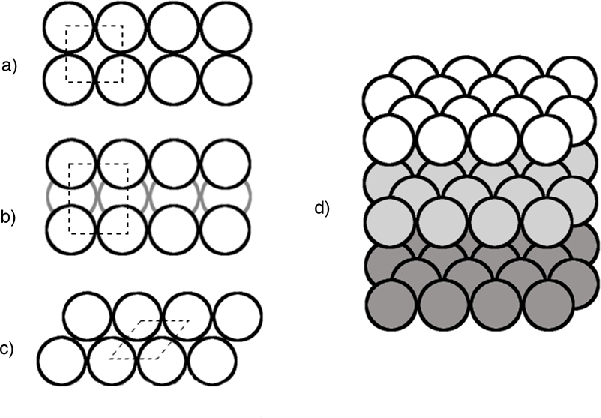
\includegraphics[width=\linewidth]{../figures/chap1/facets.pdf}
  \caption{On the left are displayed face-down views of common low-index facets
of metals (a) (100), (b) (110), and (c) (111). The dotted lines represent a
repeatable crystal unit on each facet. The light gray coloring in (b) is
illustrating the placement of that row of atoms behind the top and bottom row.
Facet (d) displays a (112) step edge. The darker shading represents separate
terraces that are displaced by one atomic height.}
\label{fig:facets}
\end{figure}

However, the presence of kinetic barriers coupled with the small size of
nanoparticles requires that not every atom on the surface will be part of a
(111) plane. As highlighted in Figure \ref{fig:facets}.d, one very common
defect observed on large crystals is that of step-edges. The (111) motif is
overwhelming present, however, there are also single atom height displacements
between plateaus. The edge atoms because of their undercoordination will
interact differently with adsorbates, potentially making those sites very
catalytically active. 

Nanoparticles and nanospheres especially have a large number of edge, kink, and
adatoms which are all of catalytic interest but are not seen on the low-index
surfaces.  However, the size of nanoparticles makes simulating them costly and
instead smaller surfaces with a large Miller index are used as a model for the
more complicated nanoparticles. Having a working knowledge of the displayed
low-energy structures is very important when considering how the metal will
interact with adsorbates because the strength of the adsorption will depend on
the displayed surfaced.


\subsubsection{Bimetallic and Supported Systems}
The displayed structure and binding properties of metal systems are directly
tied to their electronic structure and anything that perturbs the ideal system
will lead to deviations from bulk behavior. This deviation may be exactly what
is needed to tune a material for a certain catalytic process and significant
research has been directed at examining various bimetallic species including
heterogenous alloys, core-shell nanoparticles, near-surface alloys, and
supported nanoparticles. By introducing another metal or a support that will
donate or remove electron density from the system, the electronic structure can
be tuned for the desired application. Figure \ref{fig:bimetallic} shows a
number of ideal examples of these types of systems. While synthesizing these
systems can be extremely challenging, the ability to specifically tune the
catalysts for certain reactions, resistance to
poisoning\citep{Sharma:0ly,Yu:2013fr}, and cheaper costs\citep{Li:0hl,Zhao:0qf}
cannot be underestimated.

\begin{figure}[p!]
  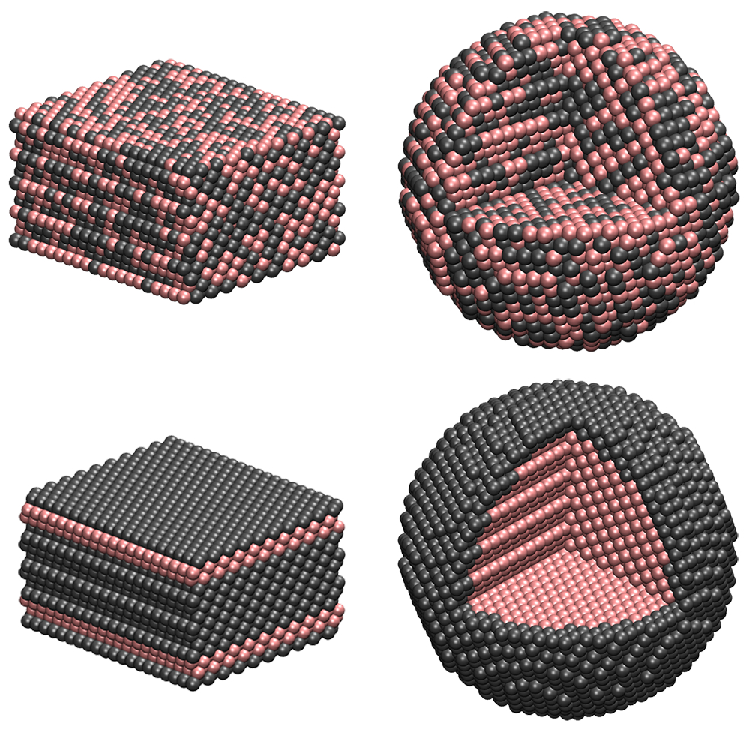
\includegraphics[width=\linewidth]{../figures/chap1/bimetallic.pdf}
\caption{The top two systems are Pd\textsubscript{0.5}Pt\textsubscript{0.5}
homogeneous alloys (Pd pink, Pt gray), with the left representing a flat plane
and the right image depicting a 30~\AA\ nanosphere. The bottom left image
displays a near-surface alloy with one layer of Pd sandwiched between layers of
Pt while the right image shows a core-shell nanosphere with a small section cut
away to allow the thickness of the shell to be observed.}
\label{fig:bimetallic} 
\end{figure}

\subsection{Dynamics}
Low-index facets of metals at room temperature will not undergo much movement
because they are already low on the potential energy surface. However, these
systems are also rarely used in real-world applications. High-index surfaces
and roughened nanoparticles have a larger number of low-coordinated surface
atoms that also tend to be more active for catalytic processes. The local
environment that enables them to bond strongly with adsorbates also can lead to
easier adatom formation and surface mobility. Repeated patterning, as seen in
step surfaces where a low-index plateau extends for some length and then
another layer of the metal is laid on top, like a staircase, can prove
especially useful because of the relatively easy characterization of the
surface.

\subsubsection{Diffusion \& Step-Wandering}
The two main types of movement that will occur on metals both involve adatoms.
Independent adatom movement is the type most likely to be seen as one particle
is ejected from a stable edge or terrace and then explores the plateau around
it. Since the strength of metallic bonding is tied to the number of nearest
neighbors, once an adatom is created and is seated on the surface, there is
often only a minimal energy barrier for it to continue exploring the surface. 

The second main type of movement involves cooperative adatom diffusion and is
better described as entire step-edges ``wandering'' on the surface. This
wandering is ultimately a collection of ejection and readsorbtion events of
surface metal atoms but it is more helpful to look at the collective motion
than all of the individual motions.

\section{Adsorbate Interactions on Metal Surfaces}
The majority of applications involving metals ultimately involve the metal
surface providing a favorable environment for some other reaction to occur,
whether that be oxidation of CO, production of \ce{H2} through a
water-gas-shift reaction, or some other mechanism that involves molecules
adsorbing to a surface. Having an accurate understanding of how adsorbates
interact with metal surfaces is thus of the utmost importance. 

\subsection{Binding Sites}
Generally, a surface with a lower index has less less electron density to
contribute to a potential adsorbate, weakening the strength of the binding.
However, the orbitals of the adsorbate also play a role in binding preference.
The three most common binding sites on a (111) facet are highlighted in Figure
\ref{fig:binding}.
\begin{figure}[p!]
  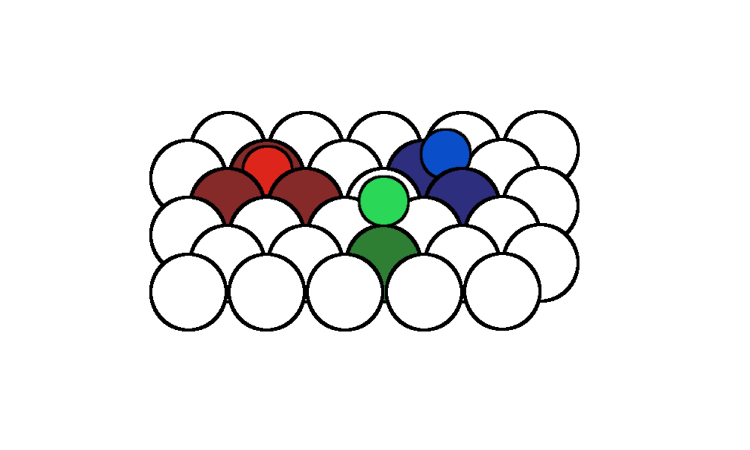
\includegraphics[width=\linewidth]{../figures/chap1/binding.pdf}
  \caption{The atop (green), bridge (blue), and three-fold hollow (red)
adsorption sites are the three most common binding sites for small molecules on
low energy surfaces. Depending on the energy levels of the adsorbate orbitals
that engage in bonding there will be varying preferences for binding sites.
Carbon monoxide's 4444 orbital is well-matched with platinum's 4444 orbital
leading to an atop preference, whereas on palladium, CO is more energetically
stable in the bridge or hollow site.}
\label{fig:binding}
\end{figure}


\subsection{Coverage Dependence}
While there might be one preferred binding site for a single adsorbate on a
metal surface, the presence of strong adsorbate-adsorbate interactions can lead
to deviations from expected behavior. While adsorbate-adsorbate interaction are
often repulsive or induce strain in the metal surface making the binding
weaker\citep{Deshlahra:2012aa} it has been shown that cooperative effects can also arise when
adsorbates are absorbed in different electronic enivornments. It has been
predicted that while \ce{CO} prefers the atop site on \ce{Pt} at low coverages,
as the coverage approaches 0.5 monolayers the binding preference changes to a
mixed atop/bridge (CHECK) configuration because of favorable dipole-dipole
interactions that result due to non-equivalent charge transfer from the Pt back
into the CO orbitals. Since the presence and configuration of adsorbates 


\subsubsection{Adsorbate Patterning}
%Image of particles adsorbed on the surface
The complex interactions between adsorbates on a surface can often lead to
large-scale patterning which can be observed with XPS (X-Ray Photoelectron
Spectroscopy), LEED (Low Energy Electron Diffraction), and other experimental
techniques. The preferred binding sites, as mentioned earlier, are dependent on
coverage, since the presence of bound adsorbates affects the energy levels of
the surface. Thus, at different coverages, different patterns are observed. For
example, \ce{CO} on \ce{Pd} at a quarter-monolayer coverage tends to be
arranged in a NUMCROSSNUM pattern. However, as the coverage increases to a
third-monolayer, the experimentally observed patterning now reveals a BLANK
pattern. Finally, one a half-monolayer of \ce{CO} is present on the (111)
surface, the preferred pattern is a c$(4\times2)$ pattern. The previously
mentioned patterns are highlighted in Figure \ref{fig:patterns}.

A good model of the adsorbate and adsorbate-metal interactions should be able
to capture some of these different patterns, however, capturing every possible
``phase change'' is incredibly complex and beyond the scope of most
investigations.

\section{Adsorbate Induced Reconstructions}
% Studies done on clean metal surfaces tend to suffer from pressure and temperature gaps
% high pressure xps, stm, spin echo helium bombardment provide some ways to mimic the environment of industrial catalysts
% Difficult to determine mechanisms because of time and spacial resolution
% DFT good at calculating relative energies for small systems, but the size of these reconstructions makes calculations expensive
% mol dyn. allows us to explore the interactions that lead to adsorbate-induced reconstructions

While metal surfaces often remain stable even when the environment is
perturbed, some situations can arise where the presence of adsorbates
sufficiently modify the potential energy surface so that a new facet is
energetically preferred. This situation might even be commonplace, but altering
the potential energy surface only solves part of the problem. The system must
also be able to overcome any kinetic barriers that would prevent the
restructuring from taking place. For systems that are started in a high-index
configuration, e.g. nanocubes and nanosphers, that are only is these
configuratios because of kinetic barriers, the introduction of adsorbates will
likely lead to a restructuring to a lower-energy structure. 

The time and length scales of these reconstruction processes vary
widely\citep{} and while current experimental techniques are able to observe
and identify the reconstructions, they are often unable to identify the
mechanisms of restructuring, which are important for designing catalysts.

\subsection{Refaceting}
%Williams papers on this, angle > ??? 
Surfaces will refacet if they were originally cut at too high of an angle. This
has been explored previously for a number of systems\citep{Jeong:1999aa} and the refaceting
will continue until RECPLACE WITH EQUATION ABOUT STABILITY. This restructuring
typically only occurs in the forward direction while the presence of adsorbates
can induce this reconstruction, a temperature increase will also likely allow
this to occur since it is most likely that there is just a kinetic barrier that
must be overcome. 

\subsubsection{Doubling}
Work by Tao {\it et al.} on a \ce{Pt} (557) surface exposed to \ce{CO} observed
a reversible reconstruction event that was directly dependent on the presence
of \ce{CO} in the system. When \ce{CO} was introduced the step-edges doubled,
but upon removal of the \ce{CO} the original (557) motif was recovered. This
reversible reconstruction strongly implies that the presence of \ce{CO}
temporarilly modifies the potential energy surface to prefer a new ground state
structure; however, the exact mechanism of this reconstruction was not deduced
at the time. This dissertation originally started as an attempt to model this
system and attemptto provide insights into the mechanism of reconstruction. 

\subsection{Island Formation}
Since catalytic reactions typically only occur at the surface, significant
research has been devoted to increasing the surface area to bulk ratio of metal
catalysts, either through catalyst supports, high-index nanostructures, or
bimetallic near surface alloys. While these systems are typically stable at low
temperatures and pressures, significant perturbations can lead to what is
effectively sintering or island-formation of one of the metals on the surface.
The interplay of surface energies and adsorbate interactions on two or more
metal surfaces can lead to surprising results.
